\documentclass[10pt,a4paper]{article}

%double si on veut une version prof et une version élève. simple si on veut une seule version.
\newcommand{\buildmode}{double}

\InputIfFileExists{version.tex}{}{}
% Version (définie par le script)
\providecommand{\version}{eleve}

\usepackage{feuilledistanciel}

%%%à modifier à chaque fois

\renewcommand{\niveau}{2nde}
\renewcommand{\chapitre}{Révisions}
\renewcommand{\numchap}{2 à 4}
\renewcommand{\theme}{Travail en distanciel}

%%% Axe gradué de -5 à 5, graduations au quart
\newcommand{\axegradue}{
\begin{center}
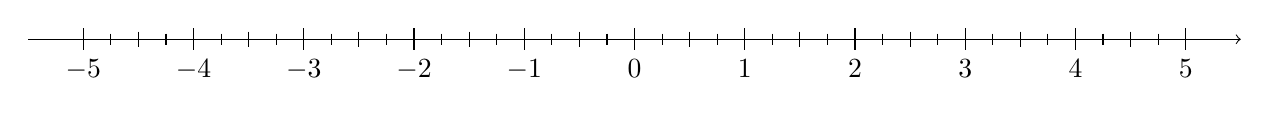
\begin{tikzpicture}[scale=1.4]
\draw[->] (-5.5,0)--(5.5,0);
\foreach \x in {-5,..., 4}{
    \draw (\x,0.1)--(\x,-0.1) node[below] {\(\x\)};
    \draw (\x+0.5,0.07)--(\x+0.5,-0.07) ;
    \foreach \minx in {0.25, 0.5, 0.75}{
        \draw (\x+\minx, 0.05)--(\x+\minx, -0.05);
    }
}
    \draw (5,0.1)--(5,-0.1) node[below] {\(5\)};
\end{tikzpicture}
\end{center}
}

%%% Droite graduée de -5 à 5, graduations à la demi-unité
\newcommand{\droitegraduee}{
\begin{center}
\begin{tikzpicture}[scale=1.4]
\draw[->] (-5.7,0)--(5.5,0);
\foreach \x in {-5,..., 5}{
    \draw (\x,0.1)--(\x,-0.1) node[below] {\(\x\)};
    \draw (\x-0.5,0.05)--(\x-0.5,-0.05);
}
\end{tikzpicture}
\end{center}
}

\begin{document}

\montitre{Révisions des premiers chapitres}

\textbf{Consignes de travail.} Traiter les sections dans l'ordre. Dans chaque section, commencer par les calculs de début de cours, sans calculatrice, puis lire attentivement le rappel de cours avant de traiter les exercices. Rédiger les réponses sur une copie, en justifiant. Chercher d'abord seul, puis lire les indications seulement en cas de blocage. Comparer enfin avec la correction et reprendre ses erreurs d'une autre couleur.

\medskip

\begin{objectifs}
Calculer une proportion et l'écrire sous forme de fraction, de nombre décimal et de pourcentage.\par\smallskip
Calculer un sous-effectif ou un effectif total à partir d'une proportion.\par\smallskip
Déterminer si un nombre est solution d'une équation ou d'une inéquation.\par\smallskip
Résoudre une équation du premier degré en détaillant les étapes.\par\smallskip
Représenter les solutions d'une inéquation sur une droite graduée et les écrire sous forme d'intervalle.\par\smallskip
Calculer des images et compléter un tableau de valeurs.\par\smallskip
Lire graphiquement une image, des antécédents et résoudre une équation \(f(x)=k\).
\end{objectifs}

\prof{
    Fiche de révision des chapitres 2 (proportions, pourcentages), 3 (équations, solutions d'inéquations) et 4 (fonctions). Les calculs de début de cours reprennent les automatismes des semaines S1 à S3 de la progression. Durée indicative : 3 h d'exercices, puis 1 h de feuille blanche.
}

%%%%%%%%%%%%%%%%%%%%%%%%%%%%%%%%%%%%%%%%%%%%%%%%%%%%%%%%%%%%%%%%%%%%%%%%%%%%%
\section{Proportions, pourcentages}

\begin{exo}[Calculs de début de cours]
Sans calculatrice.
\begin{enumerate}[leftmargin=*]
    \item Calculer :
    \begin{tasks}(3)
        \task \(3-4\)
        \task \(4-3\)
        \task \(-3+4\)
        \task \(3-(-5)\)
        \task \(-2+7-4\)
        \task \(-8-(-3)\)
    \end{tasks}
    \item Écrire plus simplement :
    \begin{tasks}(4)
        \task \(1x\)
        \task \(0x\)
        \task \(-1x\)
        \task \(3x-2x\)
    \end{tasks}
    \item Calculer la valeur de l'expression \(3x-7\) pour \(x=2\), puis pour \(x=-1\).
\end{enumerate}
\end{exo}

\begin{rappelcours}
Dans une population d'effectif total \(N\), une sous-population a pour effectif \(n\) (le \textbf{sous-effectif}). La \textbf{proportion} de cette sous-population est
\[ p=\dfrac{n}{N}. \]
Une proportion est un nombre compris entre \(0\) et \(1\). Elle peut s'écrire sous forme de fraction, de nombre décimal ou de pourcentage : \(\dfrac{3}{4}=0,75=75\,\%\).

\smallskip

\textbf{Sous-effectif :} \(n=p\times N\). \qquad \textbf{Effectif total :} \(N=\dfrac{n}{p}\). \qquad On peut aussi utiliser un tableau de proportionnalité.

\smallskip

Prendre \(t\,\%\) d'une quantité revient à la multiplier par \(\dfrac{t}{100}\) : \(30\,\%\) de \(80\) vaut \(\dfrac{30}{100}\times 80=24\).

\smallskip

\textbf{Proportions remarquables :} \(\dfrac{1}{2}=50\,\%\) ; \(\dfrac{1}{4}=25\,\%\) ; \(\dfrac{3}{4}=75\,\%\) ; \(\dfrac{1}{5}=20\,\%\) ; \(\dfrac{1}{10}=10\,\%\).
\end{rappelcours}

\begin{exo}[Guidé]
Dans une classe de seconde de \(32\) élèves, \(8\) élèves viennent au lycée à vélo. Dans une autre classe de \(25\) élèves, \(7\) élèves viennent au lycée à vélo.
\begin{enumerate}[leftmargin=*]
    \item Calculer la proportion d'élèves venant à vélo dans la première classe. Donner le résultat sous forme de fraction simplifiée.
    \item Écrire cette proportion sous forme décimale, puis sous forme de pourcentage.
    \item Pour la seconde classe, compléter le tableau de proportionnalité suivant, puis en déduire la proportion d'élèves venant à vélo sous forme de pourcentage.

    \begin{center}
    \renewcommand{\arraystretch}{1.5}
    \begin{tabular}{|l|c|c|}
        \hline
        Élèves venant à vélo & \(7\) & \(\dots\) \\ \hline
        Effectif total & \(25\) & \(100\) \\ \hline
    \end{tabular}
    \end{center}
    \item Dans quelle classe la proportion d'élèves venant à vélo est-elle la plus grande ? Justifier.
\end{enumerate}

\begin{indication}
Une proportion se calcule en divisant le sous-effectif par l'effectif total. Pour la question 3, chercher par quel nombre multiplier \(25\) pour obtenir \(100\).
\end{indication}

\checkpoint{la proportion de la question 1 est une proportion remarquable, et le pourcentage de la question 3 est compris entre \(25\,\%\) et \(30\,\%\).}
\end{exo}

\begin{exo}
Sans calculatrice, calculer :
\begin{tasks}(4)
    \task \(50\,\%\) de \(240\)
    \task \(10\,\%\) de \(70\)
    \task \(25\,\%\) de \(60\)
    \task \(75\,\%\) de \(40\)
    \task \(20\,\%\) de \(45\)
    \task le quart de \(18\)
    \task le tiers de \(27\)
    \task \(10\,\%\) de \(20\,\%\) de \(500\)
\end{tasks}
\end{exo}

\begin{exo}
Dans chacun des cas suivants, calculer la proportion et l'écrire sous forme de fraction simplifiée, de nombre décimal et de pourcentage.
\begin{enumerate}[leftmargin=*]
    \item Sur \(50\) trajets, un bus a été en retard \(12\) fois.
    \item Dans un club de \(200\) adhérents, \(30\) ont moins de \(15\) ans.
    \item Dans un championnat de \(20\) équipes, \(9\) équipes ont un entraîneur de moins de \(45\) ans.
\end{enumerate}
\end{exo}

\begin{exo}
Lors d'un match au Stade de France, à Saint-Denis, \(60\,000\) spectateurs étaient présents. \(35\,\%\) d'entre eux étaient venus en RER.
\begin{enumerate}[leftmargin=*]
    \item Calculer le nombre de spectateurs venus en RER.
    \item Lors d'un autre match, \(18\,000\) spectateurs sont venus en RER, ce qui représentait \(40\,\%\) du public. Calculer le nombre total de spectateurs.
    \item Lors d'un concert, \(13\,500\) des \(54\,000\) spectateurs sont venus en métro. Calculer la proportion de spectateurs venus en métro, sous forme de pourcentage.
\end{enumerate}
\textit{Il est possible d'utiliser un tableau de proportionnalité.}
\end{exo}

\begin{exo}[QCM][appro]
Sans calculatrice, choisir la réponse la plus vraisemblable. Justifier chaque choix par un calcul approché.
\begin{enumerate}[leftmargin=*]
    \item Parmi les \(1\,210\) élèves d'un lycée, \(298\) sont en première générale. Le pourcentage d'élèves en première générale est environ :
    \begin{tasks}(3)
        \task \(2,5\,\%\)
        \task \(24,6\,\%\)
        \task \(40,6\,\%\)
    \end{tasks}
    \item Une commune compte \(51\,980\) habitants, dont \(19,7\,\%\) ont moins de \(15\) ans. Le nombre d'habitants de moins de \(15\) ans est environ :
    \begin{tasks}(3)
        \task \(2\,640\)
        \task \(10\,240\)
        \task \(26\,400\)
    \end{tasks}
    \item Lors d'un vote, le tiers des votants a choisi A, \(30\,\%\) ont choisi B, \(\dfrac{1}{5}\) a choisi C et les autres ont choisi D. Le choix qui a recueilli le \underline{moins} de voix est :
    \begin{tasks}(4)
        \task A
        \task B
        \task C
        \task D
    \end{tasks}
\end{enumerate}
\end{exo}

\prof{
    Exercice 6 : travailler l'ordre de grandeur (\(298\approx 300\), \(1\,210\approx 1\,200\), donc environ un quart). Pour la question 3, mettre toutes les proportions sous la même forme.
}

%%%%%%%%%%%%%%%%%%%%%%%%%%%%%%%%%%%%%%%%%%%%%%%%%%%%%%%%%%%%%%%%%%%%%%%%%%%%%
\section{Équations, solutions d'inéquations}

\begin{exo}[Calculs de début de cours]
Sans calculatrice.
\begin{enumerate}[leftmargin=*]
    \item Écrire chacun des nombres suivants sous forme décimale.
    \begin{tasks}(4)
        \task \(\dfrac{1}{2}\)
        \task \(\dfrac{1}{4}\)
        \task \(\dfrac{3}{4}\)
        \task \(\dfrac{1}{5}\)
        \task \(3\times\dfrac{1}{4}\)
        \task \(5\times\dfrac{1}{2}\)
        \task \(\dfrac{7}{4}\)
        \task \(-\dfrac{2}{5}\)
    \end{tasks}
    \item Placer les nombres suivants sur l'axe gradué : \(\dfrac{3}{4}\) ; \(-\dfrac{5}{2}\) ; \(\dfrac{9}{4}\) ; \(-\dfrac{1}{4}\).
    \axegradue
    \item Calculer, en respectant les priorités opératoires :
    \begin{tasks}(3)
        \task \(2+3\times 4\)
        \task \((2+3)\times 4\)
        \task \(10-2\times(-3)\)
        \task \(18\div 3-2\times 5\)
        \task \(-4+6\div 2\)
        \task \(5-3\times(4-6)\)
    \end{tasks}
\end{enumerate}
\end{exo}

\begin{rappelcours}
Une \textbf{équation} est une égalité qui contient une inconnue, souvent notée \(x\). Un nombre est \textbf{solution} de l'équation si l'égalité est vraie lorsqu'on remplace \(x\) par ce nombre. \textbf{Résoudre} une équation, c'est trouver toutes ses solutions.

\smallskip

\textbf{Méthode :} on obtient une équation qui a les mêmes solutions en ajoutant (ou soustrayant) un même nombre aux deux membres, ou en multipliant (ou divisant) les deux membres par un même nombre \textbf{non nul}.
\[
\begin{aligned}
2x+3 &= 11\\
2x+3\textcolor{teal}{-3} &= 11\textcolor{teal}{-3}\\
2x &= 8\\
2x\textcolor{teal}{\div 2} &= 8\textcolor{teal}{\div 2}\\
x &= 4
\end{aligned}
\]

Une \textbf{inéquation} est une inégalité qui contient une inconnue. L'ensemble de ses solutions se représente sur une droite graduée et s'écrit à l'aide d'un \textbf{intervalle} : \(-2<x\leq 5\) correspond à \(]-2\ ;\ 5]\), et \(x\geq 1\) à \([1\ ;\ +\infty[\). Le crochet est tourné vers le nombre lorsque celui-ci fait partie des solutions.
\end{rappelcours}

\begin{exo}[Guidé]
On considère l'équation \((E)\ :\ 3x-5=7\), d'inconnue \(x\).
\begin{enumerate}[leftmargin=*]
    \item Le nombre \(2\) est-il solution de \((E)\) ? Pour répondre, remplacer \(x\) par \(2\) dans le membre de gauche, puis comparer le résultat avec le membre de droite.
    \item Le nombre \(4\) est-il solution de \((E)\) ? Justifier de la même façon.
    \item Résoudre l'équation \((E)\) en détaillant les étapes :
    \begin{enumerate}
        \item ajouter \(5\) aux deux membres et écrire l'équation obtenue ;
        \item diviser les deux membres par \(3\) et conclure.
    \end{enumerate}
    \item Placer la solution sur l'axe gradué de l'exercice 7.
\end{enumerate}

\begin{indication}
À chaque étape, effectuer la même opération sur les deux membres de l'égalité, comme pour garder une balance en équilibre.
\end{indication}

\checkpoint{la solution trouvée à la question 3 doit être cohérente avec les réponses aux questions 1 et 2.}
\end{exo}

\begin{exo}
Résoudre chacune des équations suivantes en détaillant les étapes, puis placer les solutions sur l'axe gradué.
\begin{tasks}(3)
    \task \(x+3=1\)
    \task \(2x-1=6\)
    \task \(4x=-3\)
    \task \(5x+2=-3\)
    \task \(-2x+1=6\)
    \task \(2x+7=8\)
\end{tasks}
\axegradue
\end{exo}

\begin{exo}
On considère l'inéquation \(-1<x\leq \dfrac{5}{2}\), d'inconnue \(x\).
\begin{enumerate}[leftmargin=*]
    \item Parmi les nombres suivants, lesquels sont solutions de cette inéquation ?
    \begin{tasks}(5)
        \task \(0\)
        \task \(-1\)
        \task \(2,5\)
        \task \(-0,99\)
        \task \(3\)
        \task \(\dfrac{5}{4}\)
        \task \(-\dfrac{3}{2}\)
        \task \(2,51\)
        \task \(1\)
    \end{tasks}
    \item Colorier sur la droite graduée l'ensemble des solutions de l'inéquation.
    \droitegraduee
    \item Écrire cet ensemble sous forme d'intervalle.
\end{enumerate}
\end{exo}

\begin{exo}
Écrire, sous forme d'intervalle, l'ensemble des solutions de chacune des inéquations suivantes.
\begin{tasks}(3)
    \task \(x<4\)
    \task \(x\geq -1\)
    \task \(0<x\leq 3\)
    \task \(-2\leq x<\dfrac{1}{2}\)
    \task \(x\leq -\dfrac{3}{4}\)
    \task \(5>x>2\)
\end{tasks}
\end{exo}

\begin{exo}[][appro]
\begin{enumerate}[leftmargin=*]
    \item Proposer trois équations différentes ayant pour solution \(-3\).
    \item Proposer une équation ayant pour solution \(\dfrac{3}{4}\).
    \item Proposer une équation dont la solution n'est pas un nombre décimal.
\end{enumerate}
\end{exo}

\prof{
    Exercice 12 : faire vérifier chaque équation proposée en remplaçant \(x\) par la valeur demandée. C'est l'occasion de revenir sur la définition d'une solution.
}

%%%%%%%%%%%%%%%%%%%%%%%%%%%%%%%%%%%%%%%%%%%%%%%%%%%%%%%%%%%%%%%%%%%%%%%%%%%%%
\section{Fonctions : image, antécédent, représentation graphique}

\begin{exo}[Calculs de début de cours]
Sans calculatrice, développer puis réduire les expressions suivantes.
\begin{tasks}(3)
    \task \(3(x+4)\)
    \task \(-2(x-5)\)
    \task \(-(4-x)\)
    \task \(5(2x-1)-3x\)
    \task \(x(x+3)\)
    \task \(-4(-2x+3)\)
\end{tasks}
\end{exo}

\begin{rappelcours}
Une \textbf{fonction} \(f\) associe à chaque nombre \(x\) de son \textbf{ensemble de définition} \(\mathcal{D}_f\) un \textbf{unique} nombre, noté \(f(x)\).

\smallskip

Si \(f(a)=b\) : on dit que \(b\) est \textbf{l'image} de \(a\) par \(f\), et que \(a\) est \textbf{un antécédent} de \(b\) par \(f\). Un nombre a une seule image, mais un nombre peut avoir zéro, un ou plusieurs antécédents.

\smallskip

La \textbf{courbe représentative} \(\mathcal{C}_f\) est l'ensemble des points de coordonnées \((x\ ;\ f(x))\). Un point \(M(a\ ;\ b)\) appartient à \(\mathcal{C}_f\) si et seulement si \(f(a)=b\).

\smallskip

\textbf{Lectures graphiques :} l'image de \(a\) se lit sur l'axe des ordonnées ; les antécédents de \(b\) sont les abscisses des points de \(\mathcal{C}_f\) d'ordonnée \(b\). Résoudre l'équation \(f(x)=k\), c'est trouver tous les antécédents de \(k\).
\end{rappelcours}

\begin{exo}[Guidé]
On considère la fonction \(f\) définie sur l'intervalle \([-1\ ;\ 3]\) par \(f(x)=x^2-2x-1\).
\begin{enumerate}[leftmargin=*]
    \item Calculer \(f(2)\) en détaillant le calcul.
    \item Calculer \(f(-1)\) en détaillant le calcul.
    \item Compléter le tableau de valeurs suivant.

    \begin{center}
    \renewcommand{\arraystretch}{2}
    \begin{tabular}{|*{8}{c|}}
        \hline
        \(x\) & \(-1\) & \(-\dfrac{1}{2}\) & \(0\) & \(1\) & \(2\) & \(\dfrac{5}{2}\) & \(3\) \\
        \hline
        \(f(x)\) & & & & & & & \\
        \hline
    \end{tabular}
    \end{center}
    \item Placer les points du tableau dans le repère ci-dessous, puis tracer la courbe \(\mathcal{C}_f\).

    \begin{center}
    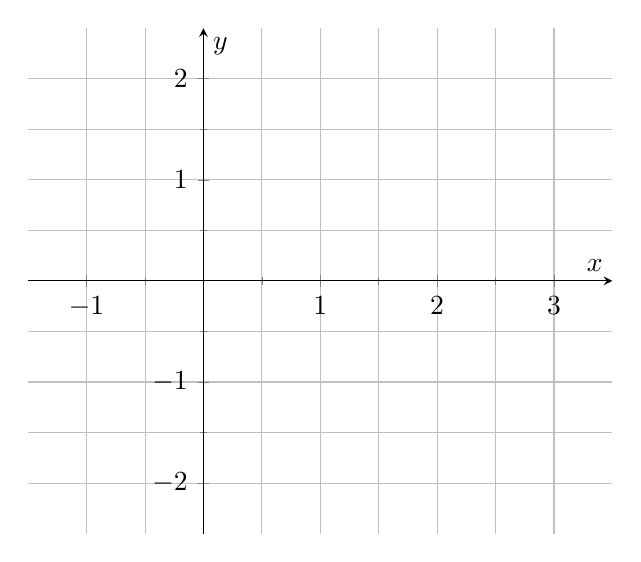
\begin{tikzpicture}
    \begin{axis}[
        axis lines=middle,
        xmin=-1.5, xmax=3.5,
        ymin=-2.5, ymax=2.5,
        grid=both,
        minor tick num=1,
        xtick={-1,0,...,3},
        ytick={-2,-1,...,2},
        xlabel={\(x\)},
        ylabel={\(y\)},
        width=9cm,
        height=8cm
    ]
    \end{axis}
    \end{tikzpicture}
    \end{center}
    \item Le point \(A(1\ ;\ -2)\) appartient-il à \(\mathcal{C}_f\) ? Et le point \(B(3\ ;\ 1)\) ? Justifier par le calcul.
\end{enumerate}

\begin{indication}
Remplacer \(x\) par la valeur demandée en écrivant des parenthèses : \(f(-1)=(-1)^2-2\times(-1)-1\). Attention : \((-1)^2=1\) et \(-2\times(-1)=2\).
\end{indication}

\checkpoint{on doit obtenir \(f\left(-\dfrac{1}{2}\right)=f\left(\dfrac{5}{2}\right)\).}
\end{exo}

\begin{exo}
On considère une fonction \(f\) dont la représentation graphique est donnée ci-dessous.

\begin{center}
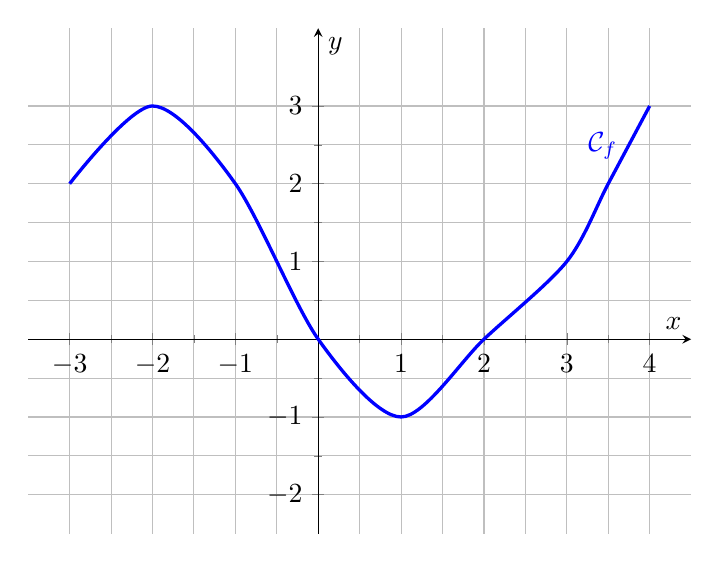
\begin{tikzpicture}
\begin{axis}[
    axis lines=middle,
    xmin=-3.5, xmax=4.5,
    ymin=-2.5, ymax=4,
    grid=both,
    minor tick num=1,
    xtick={-3,-2,...,4},
    ytick={-2,-1,...,3},
    xlabel={\(x\)},
    ylabel={\(y\)},
    width=10cm,
    height=8cm
]
\addplot[blue, very thick, smooth] coordinates {(-3,2)(-2,3)(-1,2)(0,0)(1,-1)(2,0)(3,1)(3.5,2)(4,3)}
node[pos=0.95, left] {\(\mathcal{C}_f\)};
\end{axis}
\end{tikzpicture}
\end{center}

\begin{enumerate}[leftmargin=*]
    \item Donner l'ensemble de définition de \(f\).
    \item Donner les images de \(-2\), de \(0\) et de \(2\) par \(f\).
    \item Donner les éventuels antécédents de \(0\), puis de \(-2\).
    \item Résoudre graphiquement l'équation \(f(x)=2\).
    \item Résoudre graphiquement l'équation \(f(x)=3\).
\end{enumerate}
\textit{Faire apparaître les lectures graphiques à l'aide de pointillés.}
\end{exo}

\begin{exo}
Une fonction \(g\) est définie sur l'intervalle \([-3\ ;\ 3]\). On connaît seulement le tableau de valeurs suivant.

\begin{center}
\renewcommand{\arraystretch}{2}
\begin{tabular}{|*{8}{c|}}
    \hline
    \(x\) & \(-3\) & \(-2\) & \(-1\) & \(0\) & \(1\) & \(2\) & \(3\) \\
    \hline
    \(g(x)\) & \(4\) & \(-1\) & \(0\) & \(\dfrac{5}{2}\) & \(-1\) & \(4\) & \(\dfrac{1}{2}\) \\
    \hline
\end{tabular}
\end{center}

\begin{enumerate}[leftmargin=*]
    \item Donner l'image de \(0\) par \(g\), puis la valeur de \(g(-1)\).
    \item D'après le tableau, donner les antécédents de \(4\), puis ceux de \(-1\).
    \item D'après le tableau, donner une solution de l'équation \(g(x)=\dfrac{1}{2}\).
    \item Ce tableau permet-il de connaître \(g(1,5)\) ? Justifier.
\end{enumerate}
\end{exo}

\begin{exo}[Vrai ou faux][appro]
Dire si chacune des affirmations suivantes est vraie ou fausse, en justifiant.
\begin{enumerate}[leftmargin=*]
    \item Un nombre peut avoir deux images différentes par une même fonction.
    \item Si \(f(3)=5\), alors \(3\) est un antécédent de \(5\) par \(f\).
    \item Si deux nombres différents ont la même image, alors \(f\) n'est pas une fonction.
    \item On considère la fonction \(h\) définie par \(h(x)=\dfrac{x}{x-2}\). Le nombre \(2\) a une image par \(h\).
\end{enumerate}
\end{exo}

\prof{
    Exercice 17, question 4 : faire calculer quelques images (\(h(0)\), \(h(4)\)) avant de tester \(x=2\). Conclure sur l'ensemble de définition de \(h\).
}

%%%%%%%%%%%%%%%%%%%%%%%%%%%%%%%%%%%%%%%%%%%%%%%%%%%%%%%%%%%%%%%%%%%%%%%%%%%%%
\section{Problèmes}

Les problèmes suivants mélangent les notions des trois sections précédentes.

\begin{exo}[Un rectangle]
Un rectangle a pour longueur \(2x+3\) et pour largeur \(x\), en centimètres, où \(x\) est un nombre strictement positif. On note \(P(x)\) son périmètre.
\begin{enumerate}[leftmargin=*]
    \item Montrer que \(P(x)=6x+6\).
    \item Compléter le tableau de valeurs suivant.

    \begin{center}
    \renewcommand{\arraystretch}{1.5}
    \begin{tabular}{|*{6}{c|}}
        \hline
        \(x\) & \(1\) & \(2\) & \(3\) & \(4\) & \(5\) \\ \hline
        \(P(x)\) & & & & & \\ \hline
    \end{tabular}
    \end{center}
    \item Résoudre l'équation \(6x+6=30\). Interpréter le résultat dans le contexte de l'exercice.
    \item Calculer l'aire du rectangle pour cette valeur de \(x\).
\end{enumerate}

\begin{indication}
Le périmètre d'un rectangle est égal à \(2\times\text{longueur}+2\times\text{largeur}\). Penser à développer.
\end{indication}
\end{exo}

\begin{exo}[Deux formules d'abonnement]
Une salle de sport de Saint-Denis propose deux formules mensuelles :
\begin{itemize}
    \item \textbf{formule A} : un forfait de \(30\) \euro{} par mois, avec un nombre de séances illimité ;
    \item \textbf{formule B} : \(6\) \euro{} par mois, auxquels s'ajoutent \(4\) \euro{} par séance.
\end{itemize}
On note \(x\) le nombre de séances dans le mois et \(B(x)\) le prix payé, en euros, avec la formule B. On a donc \(B(x)=4x+6\).
\begin{enumerate}[leftmargin=*]
    \item Calculer \(B(3)\) et \(B(8)\). Interpréter ces résultats.
    \item Compléter le tableau de valeurs suivant.

    \begin{center}
    \renewcommand{\arraystretch}{1.5}
    \begin{tabular}{|*{7}{c|}}
        \hline
        \(x\) & \(0\) & \(2\) & \(4\) & \(6\) & \(8\) & \(10\) \\ \hline
        \(B(x)\) & & & & & & \\ \hline
    \end{tabular}
    \end{center}
    \item Résoudre l'équation \(4x+6=30\). Interpréter le résultat.
    \item À l'aide du tableau, indiquer pour quels nombres de séances la formule B est la plus avantageuse.
    \item En septembre, la salle accorde une réduction de \(15\,\%\) sur la formule A.
    \begin{enumerate}
        \item Calculer le montant de la réduction, puis le nouveau prix de la formule A.
        \item Une personne prévoit \(5\) séances en septembre. Quelle formule doit-elle choisir ? Justifier.
    \end{enumerate}
\end{enumerate}
\end{exo}

\prof{
    Exercice 19 : la fonction \(B\) est affine, mais ce vocabulaire n'est pas attendu ici (chapitre 6). La question 4 se traite par lecture du tableau, sans résolution d'inéquation.
}

%%%%%%%%%%%%%%%%%%%%%%%%%%%%%%%%%%%%%%%%%%%%%%%%%%%%%%%%%%%%%%%%%%%%%%%%%%%%%
\section{Bilan}

Réaliser une très longue feuille blanche (1 h, soit \(3\times 20\) minutes) sur ce qui a été fait dans cette feuille. On rappelle que les objectifs de cette feuille étaient les suivants :

\medskip

Calculer une proportion et l'écrire sous forme de fraction, de nombre décimal et de pourcentage.\par\smallskip
Calculer un sous-effectif ou un effectif total à partir d'une proportion.\par\smallskip
Déterminer si un nombre est solution d'une équation ou d'une inéquation.\par\smallskip
Résoudre une équation du premier degré en détaillant les étapes.\par\smallskip
Représenter les solutions d'une inéquation sur une droite graduée et les écrire sous forme d'intervalle.\par\smallskip
Calculer des images et compléter un tableau de valeurs.\par\smallskip
Lire graphiquement une image, des antécédents et résoudre une équation \(f(x)=k\).

\prof{
    Feuille blanche : rappeler qu'elle est personnelle, sans cours ni fiche. Possibilité de la faire en trois temps de 20 minutes, en relisant la fiche entre deux temps.
}

\end{document}
